\section{Introduction}
\begin{figure}
    \centering
    \includegraphics[width=\linewidth]{figs/autolibra_teaser.pdf}
    \caption{Caption}
    \label{fig:enter-label}
\end{figure}
\begin{wrapfigure}[17]{r}{0.4\textwidth} 
\vspace{-64pt}
   \centering
   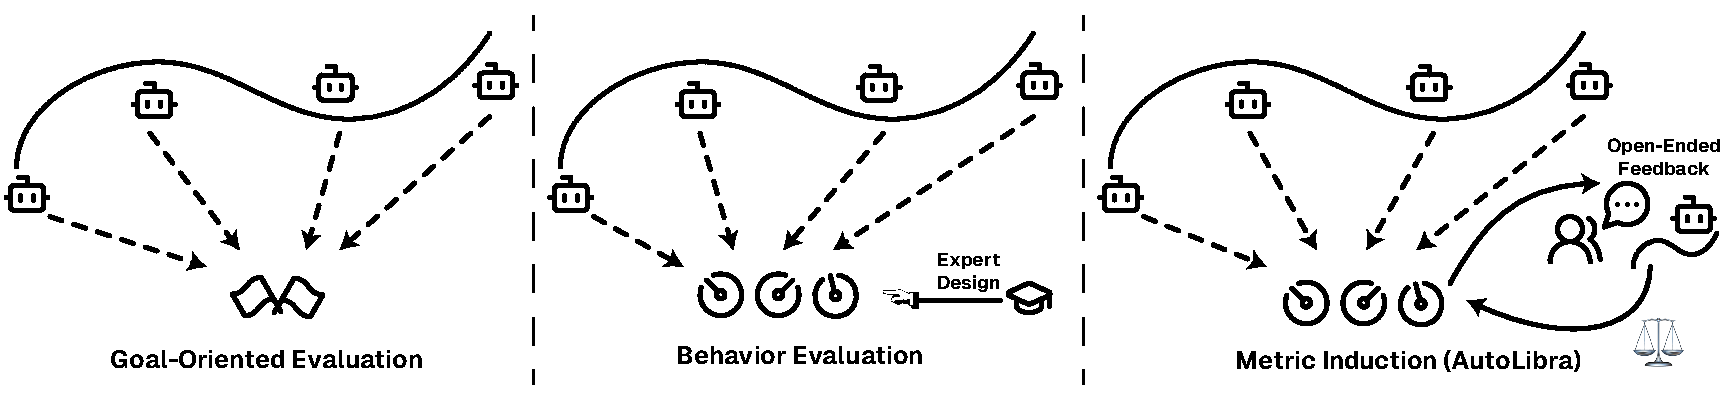
\includegraphics[width=0.4\textwidth]{figs/autolibra.pdf}
   \vspace{-10pt}
   \caption{AutoLibra provides \\ 
    behavioral evaluation on agent performance
    through automatic metric induction based on human feedback and agent trajectories.}
\end{wrapfigure}

Current AI agents acquire skills from demonstrations and trial and errors.
In contrast, efficient human learners internalize open-ended feedback from others into self-regulation dimensions
\citep{pintrich2002development,nicol2006formative},  or ``metrics'', which offer structured criteria for self-reflection on one's 
strengths and weaknesses and guidelines for incremental self-improvement.
Can we build AI systems that draw inspiration from this process to efficiently make use human feedback for agent evaluation and improvement?

\begin{figure}[!b]
    \centering
    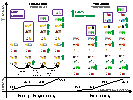
\includegraphics[width=\textwidth]{figs/autolibra-teaser.pdf}
    \vspace{-10pt}
    \caption{AutoLibra iteratively discovers new optimization targets throughout the agent optimization process. \diyi{this figure needs more explanation currently, there is not much info for readers to understand Fig 2 at this moment. you can't expect readers to finish reading this paper and then coming back to Fig 2 to digest it.}}
    \label{fig:autolibra-training}
\end{figure}

   
There are two major paradigms for evaluation and reward modeling of large language model (LLM) agents currently exist: (1) goal-oriented evaluation --
\emph{whether the agents have fulfilled the given task},
\emph{e.g.} benchmarks \citep{zhouwebarena,jimenezswe,chan2024mle,paglieri2024balrog} and reward
modeling approaches \citep{pan2024autonomous,chen2025scaling,choudhury2025process}
and (2) behavior evaluation -- \emph{how well the agents do on heuristically designed dimensions},
\emph{e.g.} social agent and human-agent interaction benchmarks \citep{zhousotopia,shao2024collaborative}
and agent failure mode analysis \citep{pan2025why,zhang2023effects,yang2023behavioral}.
\diyi{is this categorization based on any prior work, or did we introduce this categorization? is "behavior" eval more about process or procedural eval, and goal oriented more about task success or completion? }
\textit{Goal-oriented evaluation} is designed to be verifiable through considering, but is not fine-grained
or comprehensive enough to diagnose agents' behavior problems or find bottlenecks for improvements \citep{yehudai2025survey}.  
Although the above can be complemented with behavior evaluation, this method requires manual design of metrics based on top-down heuristics
\citep{zhousotopia}, or thematic analysis of the agent's behavior \citep{shao2024collaborative,pan2025why}.
This manual design process is time-consuming and labor-intensive \diyi{you may want to be clear about this (e.g., manual design of these metrics); otherwise you current framework also involves human annotation or human provided feedback}, requiring expert annotations and classification, limiting its scalability. 

In this paper, we introduce AutoLibra \protect\includegraphics[height=1em]{figs/scale.png},
a metric induction method, as a novel agent evaluation framework
that mitigates the limitations of current evaluation paradigms.
This method offers behavior evaluation for agents, with the following advantages:
(1) it provides multi-dimensional behavior evaluation that is fine-grained but requires no manual design of metrics, \diyi{there is a shift from "no manual design of metrics" to "require manual or human feedback towards the process". at some time, you need to balance the tradeoff here, as it is not that autolibra is simply human-effort-free.}
(2) it can be applied to a broad spectrum of agents and tasks, and
(3) induced metrics are fully explainable and interpretable by humans.



Inspired by the code-theme steps of thematic analysis conducted by experts
in social sciences \citep{braun2006using},
we design the AutoLibra extraction process as two steps:
(1) \emph{grounding}: ground every aspect of human feedback into a slice of the entire agent trajectory,
and (2) \emph{clustering}: cluster the aspects of all trajectories into multiple clusters of similar behaviors
to summarize into metrics. For example, in the context of web agents, grounding
``\textsf{If you find that the button is disabled, do not click it again}'' maps the feedback to an agent trajectory slice
``\texttt{action: click[1234]} \texttt{obs: no change} \texttt{action: click[1234]}''. Similar slices in which agents repeatedly interact with disabled elements could be clustered into a metric \texttt{ interacted-valid element}. 


The AutoLibra evaluation process is designed to provide a closed-loop feedback signal for both the extraction process
and the LLM-as-a-Judge step. The agent trajectories used in the extraction process are scored by the LLM-as-a-Judge based
on the metrics induced by the extraction process. The evaluation process then tries to match the detected agent traits,
\emph{e.g.} \texttt{interact-valid-element}: \texttt{negative}, with the human feedback aspects.
In this way, we can meta-evaluate \emph{coverage} of the detected traits and \emph{redundancy} of the metrics,
i.e., what proportion of the aspects in the human feedback are detected as agent traits,
and what proportion of the detected traits are not mentioned by humans, respectively. These two meta-metrics are used in selecting
metrics from candidates proposed in the extraction process.



With AutoLibra, our aim is to answer the following research questions:

\textbf{RQ1:} Can LLMs serve as a proxy \diyi{i didn't follow this RQ} for humans when used in agent behavior thematic analysis,
    behavior evaluation, and meta-evaluation of the LLM-as-a-Judge results?

\textbf{RQ2:}    What are the differences between behavior evaluation metrics \diyi{why is the metrics dervied by autolibra "behavior" not goal oriented?} induced by AutoLibra and those designed by human experts?

\textbf{RQ3:}  Can AutoLibra improve agent performance by providing fine-grained behavior evaluation for human agent engineers and agent learning algorithms?


Experiments within multiple agent domains, including collaborative agents \citep{shao2024collaborative}, social agents
\citep{zhousotopia}, web agents \citep{zhouwebarena,he2024webvoyager}, and text game agents \citep{paglieri2024balrog,cloos2024babaaibreakrules}, 
demonstrate that AutoLibra is able to induce fine-grained and interpretable metrics with high coverage and low redundancy on unseen human feedback.

We also find that new metrics can be iteratively discovered by AutoLibra through the agent optimization process,
and provide salient and human-interpretable optimization signals that are useful for improving the performance of agents in different tasks, with task completion rate improvements of up to 20\% observed over baseline agents.



\diyi{i think the Introduction still needs some work. First, why do we even want to do metric induction? Why can't we ask humans to come up with metrics? Why do we prefer to let humans provide feedback into the process, and then induce the metrics from it? It is okay to start with cons of existing metrics, but then we need to discuss how we should mitigate issues of prior evaluation metrics. We want to leverage human feedback because it is easier for humans to provide natural language feedback in terms of how the agent is doing, compared to asking humans to design metrics. Such procedural metrics give more insights compared to an overall task level signal. I don't know whether we want to draw any connections of these metrics derived by autolibra compared to behavior or goal oriented metrics, as it might be possible that some of these are behavior while others could be indicative of goals.}